\documentclass[10pt,twocolumn]{article}

\usepackage[letterpaper,top=0.58in,bottom=0.70in,left=0.64in,right=0.64in,columnsep=0.25in]{geometry}
\usepackage{amsmath,amssymb,bm}
\usepackage{booktabs}
\usepackage{microtype}
\usepackage{setspace}
\usepackage{tikz}
\usetikzlibrary{arrows.meta,calc,positioning}
\usepackage[font=small,labelfont=bf]{caption}
\usepackage[hidelinks]{hyperref}
\usepackage{cite}
\usepackage{balance}

% Readability pass retained from v3.x.
\setstretch{1.06}
\setlength{\parindent}{1.0em}
\setlength{\parskip}{0.16em plus 0.03em minus 0.02em}
\setlength{\columnsep}{0.25in}
\setlength{\columnseprule}{0pt}
\setlength{\jot}{5pt}
\setlength{\abovedisplayskip}{7.5pt plus 2pt minus 2pt}
\setlength{\belowdisplayskip}{7.5pt plus 2pt minus 2pt}
\setlength{\abovedisplayshortskip}{5pt plus 2pt minus 1pt}
\setlength{\belowdisplayshortskip}{6pt plus 2pt minus 1pt}
\setlength{\textfloatsep}{11pt plus 3pt minus 2pt}
\setlength{\floatsep}{10pt plus 3pt minus 2pt}
\setlength{\intextsep}{10pt plus 3pt minus 2pt}
\captionsetup{skip=5pt}
\emergencystretch=2em
\raggedbottom
\pagestyle{plain}

\newcommand{\TEF}{\mathrm{TEF}}
\newcommand{\Vol}{\operatorname{Vol}}
\newcommand{\geom}{\mathrm{geom}}
\newcommand{\Exp}{\mathrm{exp}}

\begin{document}

\twocolumn[
\begin{@twocolumnfalse}
\begin{center}
{\LARGE\bfseries From a Gravity-Calibrated Helix to a Conditional\\[3pt]
Fine-Structure Correspondence\par}
\vspace{0.62em}
{\large Xiaodan Wu\par}
\vspace{0.20em}
{\small Independent Researcher\par}
\vspace{0.12em}
{\small \texttt{xiaodan@theemergentframe.org}\par}
{\small \url{https://theemergentframe.org}\quad |\quad ORCID: \href{https://orcid.org/0009-0005-5892-0293}{0009-0005-5892-0293}\par}
{\small DOI: \href{https://doi.org/10.5281/zenodo.22117153}{10.5281/zenodo.22117153}\par}
\vspace{0.25em}
{\small August 2026\par}
\end{center}

\vspace{0.45em}
\begingroup
\setstretch{1.045}
\noindent\textbf{Abstract.}
We report a frozen numerical correspondence generated from the dimensionless helix
parameter established in the preceding TEF preprint.  That construction uses the measured
Newton constant to calibrate a primitive radius,
$R_G=\sqrt{hG/(8\pi c^3)}=\ell_P/2$, and then fixes the dimensionless shape by one-cycle
phase closure, $q\sqrt{1+q^2}=2/\pi$, giving $q=0.5563241800\ldots$ without electroweak
input.  The present paper introduces the scale-free helical path excess
$\delta_{\rm h}=\sqrt{1+q^2}-1$ and explores a conditional spinorial completion of a framed
state by $SU(2)\simeq S^3$.  We explicitly separate this completion, the minimal Hopf-coordinate
identification $\eta=\beta$ with $q=\tan\beta$, and the choice of a unit round $S^3$ with its
unnormalized Riemann volume measure.  Under these assumptions the Hopf-band volume fraction
is exactly $\sin^2\beta$, while the unit-sphere volume is $2\pi^2$.  We then \emph{postulate,
not derive}, the electromagnetic correspondence
$\alpha_{\TEF}=\delta_{\rm h}/(2\pi^2)$, obtaining
$\alpha_{\TEF}^{-1}=136.7621663\ldots$, about $0.2002\%$ from the 2022 CODATA recommended
low-energy value.  The factor $1/(2\pi^2)$ is not claimed to follow physically from probability
normalization: it depends on the metric scale and measure convention unless a future TEF action
fixes them.  The result is therefore presented as a frozen, gravity-anchored geometric
correspondence with explicit theoretical failure conditions, rather than a derivation or precision
prediction of QED.  Its main purpose is to expose a concrete possible map
$G\rightarrow R_G\rightarrow q\rightarrow\alpha_{\TEF}$ and, equivalently after calibration,
a simple expression of the fine-structure candidate in terms of the inherited $q$.
\endgroup
\vspace{0.9em}
\hrule
\vspace{0.9em}
\end{@twocolumnfalse}
]

\section{Introduction}

The fine-structure constant is the dimensionless electromagnetic coupling.  In SI notation,
\begin{equation}
\alpha=\frac{e_{\rm SI}^2}{4\pi\varepsilon_0\hbar c}.
\end{equation}
The 2022 CODATA recommended low-energy value is \cite{Mohr2025,NISTalpha}
\begin{equation}
\alpha(0)^{-1}=137.035999177(21).
\label{eq:alpha0}
\end{equation}
This value is a recommended adjustment informed by several precision inputs, rather than a
single direct experiment.  Electron magnetic-moment measurements and atom-recoil determinations
provide complementary high-precision routes to the same low-energy coupling.

Beyond the Thomson limit, the electromagnetic coupling runs through vacuum polarization and
radiative corrections.  Electroweak quantities conventionally described by a weak mixing angle
are likewise scale- and scheme-dependent \cite{PDG2026}.  Importantly for the present paper,
modern lattice-QCD calculations treat the hadronic running of the electromagnetic coupling and the
electroweak mixing angle within one correlated framework.  C\`e \emph{et al.} computed both
$\Delta\alpha_{\rm had}$ and the hadronic contribution to the running weak angle from vacuum
polarization functions \cite{Ce2022}; Conigli \emph{et al.} recently extended this program to
permille-level precision for spacelike virtualities up to the multi-GeV regime and a high-precision
continuation toward the $Z$ pole \cite{Conigli2026}.  These results reinforce a basic constraint on
any TEF interpretation: $\alpha$ and $\theta_W$ cannot be assigned unrelated scale corrections.
Consequently, a proposed geometric number can be compared directly with Eq.~\eqref{eq:alpha0},
but a claim that it is an ultraviolet or ``bare'' seed requires a specified matching scale,
renormalization prescription, and common electroweak dynamics.

Attempts to explain $\alpha$ by geometric or algebraic constants have a long history.  The main
methodological danger is not arithmetic error but post-hoc functional choice: sufficiently many
simple combinations can approximate a known number.  The criticism of Wyler-type formulae
remains relevant in this respect \cite{Robertson1971}.  The present work therefore separates two
facts that must not be conflated.  First, the parameter $q$ was already frozen in an earlier publicly
released TEF ansatz and is not reoptimized here \cite{WuCompanion}.  Second, the map from $q$ to
$\alpha$ proposed below was recognized after comparison with electromagnetic data and therefore
carries a look-elsewhere burden of its own.

The preceding TEF paper, \emph{A Helical Spacetime Ansatz Linking the Planck Scale and
Electroweak Mixing}, version 5.1, develops a gravity-calibrated helical spacetime ansatz and a
candidate primitive geometric reference angle for weak mixing \cite{WuCompanion}.  The present
paper asks a narrower continuation question: can the same frozen helical shape support a simple,
explicitly conditional correspondence with the electromagnetic coupling?

This question is adjacent to, but distinct from, several mainstream research programs in which
low-energy couplings may be controlled by deeper structure.  Quantum-gravity fixed points can
constrain gauge couplings in asymptotic-safety scenarios \cite{EichhornHeldWetterich}.  Recent
functional-renormalization-group work continues to calculate gravitational contributions to gauge-
and Yukawa-coupling beta functions and to quantify their gauge- and regulator-dependence
\cite{Giacometti2026}.  Other work asks whether familiar gauge symmetries or spacetime itself may
be emergent rather than fundamental \cite{Bass2026,Addazi2024,Addazi2025}.  These approaches do
not validate TEF.  They establish only that the broader question---whether measured gauge parameters
can encode ultraviolet geometric or gravity-related structure---is a recognizable field-theoretic one.

\section{Inherited Result I: the gravity-calibrated helix}
\label{sec:inherited}

The present paper inherits the three postulates and two geometric propositions of
Ref.~\cite{WuCompanion}.  They are summarized here so that the input chain is self-contained.
A local spatial line is represented by the right-handed helix
\begin{equation}
\bm r(\phi)=\bigl(R\cos\phi,\;R\sin\phi,\;a\phi\bigr),
\qquad
q\equiv\frac{a}{R}=\tan\beta.
\label{eq:helix}
\end{equation}
The earlier paper first calibrates the transverse scale through
\begin{equation}
G=\frac{8\pi c^3R^2}{h},
\label{eq:Gcalibration}
\end{equation}
so that the measured Newton constant gives
\begin{equation}
R_G=\sqrt{\frac{hG}{8\pi c^3}}=\frac{\ell_P}{2}.
\label{eq:RG}
\end{equation}
Equation~\eqref{eq:Gcalibration} is a TEF calibration postulate, not a prediction of $G$.

A complete turn has axial extension and internal helical length
\begin{align}
P&=2\pi qR,\\
L_{\rm cyc}&=2\pi R\sqrt{1+q^2}.
\label{eq:cyclelengths}
\end{align}
The earlier ansatz assigns the gravitational line-tension scale $c^4/G$ to the net axial
extension,
\begin{equation}
E_{\rm cyc}=\frac{c^4}{G}P,
\end{equation}
while the internal traversal time is
\begin{equation}
T_{\rm cyc}=\frac{L_{\rm cyc}}{c}.
\end{equation}
Its third postulate requires one primitive cycle to close its quantum phase,
\begin{equation}
\frac{E_{\rm cyc}T_{\rm cyc}}{\hbar}=2\pi.
\label{eq:phaseclosure}
\end{equation}
Before the gravity calibration is inserted, Eqs.~\eqref{eq:Gcalibration}--\eqref{eq:phaseclosure}
lead to
\begin{equation}
q\sqrt{1+q^2}=X_G,
\qquad
X_G\equiv\frac{hG}{4\pi^2c^3R^2},
\label{eq:XG}
\end{equation}
and therefore
\begin{equation}
q(G,h,c;R)=
\sqrt{\frac{\sqrt{1+4X_G^2}-1}{2}}.
\label{eq:qG}
\end{equation}
This equation retains the explicit gravitational ancestry of the dimensionless shape.
With $R=R_G$, however, the dimensional constants cancel and
\begin{equation}
q\sqrt{1+q^2}=\frac{2}{\pi},
\label{eq:qconstraint}
\end{equation}
so that
\begin{equation}
q^2=\frac{-1+\sqrt{1+16/\pi^2}}{2},
\qquad
q=0.556324180045\ldots.
\label{eq:qclosed}
\end{equation}
The corresponding intrinsic angle is
\begin{align}
\beta&=\arctan q=29.0882455^\circ,\\
\sin^2\beta&=0.2363477652\ldots.
\label{eq:beta}
\end{align}
No electromagnetic or weak-mixing datum is used in Eqs.~\eqref{eq:Gcalibration}--\eqref{eq:beta}.
The important qualification is that $G$ calibrates the microscopic scale, while the final
calibrated shape is dimensionless and no longer depends numerically on the measured magnitude of
$G$.

\begin{figure}[t]
\centering
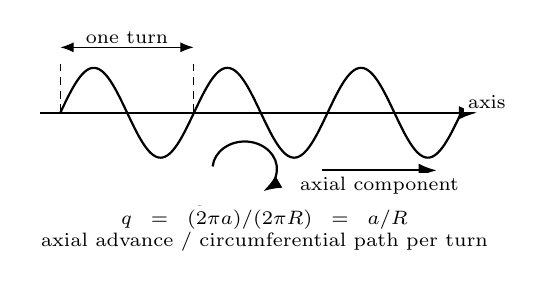
\begin{tikzpicture}[x=0.73cm,y=0.62cm,>=Latex,font=\scriptsize]
  \draw[->,thick] (-0.35,0) -- (7.25,0);
  \node[anchor=west,fill=white,inner sep=1.3pt] at (7.02,0.23) {axis};

  \draw[domain=0:18.85,samples=260,smooth,variable=\t,thick]
    plot ({0.37*\t},{0.92*sin(57.2958*\t)});

  \draw[densely dashed] (0,0) -- (0,1.00);
  \draw[densely dashed] (2.32,0) -- (2.32,1.00);
  \draw[<->] (0,1.34) -- (2.32,1.34)
    node[midway,above,fill=white,inner sep=1.3pt] {one turn};

  \draw[->,thick] (4.55,-1.18) -- (6.55,-1.18);
  \node[anchor=north,fill=white,inner sep=1.5pt]
    at (5.55,-1.23) {axial component};

  \draw[->,thick] (2.65,-1.10)
    arc[start angle=175,end angle=-55,radius=0.56];
  \node[anchor=north,fill=white,inner sep=1.5pt]
    at (2.45,-1.82) {circulation};

  \node[align=center,text width=5.9cm,fill=white,inner sep=1.6pt]
    at (3.55,-2.42)
    {$q=(2\pi a)/(2\pi R)=a/R$\\axial advance / circumferential path per turn};
\end{tikzpicture}
\caption{Schematic projection of the inherited TEF helix.  The drawing is kinematic and
not to scale.  The same frozen shape parameter $q$ is used throughout the present paper.}
\label{fig:helix}
\end{figure}

\section{Proposition 1: helical path excess}

For one turn, the circumferential projection has length $L_{\rm circ}=2\pi R$, while the
helical path has length $L_{\rm helix}=2\pi R\sqrt{1+q^2}$.  Their scale-free fractional excess is
\begin{equation}
\boxed{
\delta_{\rm h}\equiv
\frac{L_{\rm helix}-L_{\rm circ}}{L_{\rm circ}}
=\sqrt{1+q^2}-1.
}
\label{eq:delta}
\end{equation}
For the inherited value of $q$,
\begin{equation}
\delta_{\rm h}=0.144332378858\ldots.
\end{equation}
Its small-$q$ expansion begins at second order,
\begin{equation}
\delta_{\rm h}
=\frac{q^2}{2}-\frac{q^4}{8}+\mathcal O(q^6).
\label{eq:smallq}
\end{equation}
This makes $\delta_{\rm h}$ a simple intensity-like scalar associated with the orthogonal helical
component, but no QED amplitude or action coefficient is derived from Eq.~\eqref{eq:delta}.

\section{Postulate S1: spinorial orientation completion}
\label{sec:s1}

A circular helix embedded in ordinary three-space does not imply $S^3$.  The present paper makes
an additional structural assumption: a framed TEF state retains a $4\pi$ orientation periodicity,
so that its orientation variable is lifted from $SO(3)$ to the double cover $SU(2)$.  As a manifold,
the unit-quaternion representation of $SU(2)$ is $S^3$ \cite{Nakahara2003}.

This completion concerns the configuration/orientation variable of a framed state.  It is distinct
from the $2\pi$ quantum phase closure in Eq.~\eqref{eq:phaseclosure}: the latter closes one $U(1)$
phase cycle, whereas the former concerns a double-covered rotational configuration space.  The
present paper does not derive why TEF must retain the $SU(2)$ double-cover information; this is
Postulate S1.

It is also important to distinguish three related but nonidentical objects: a group element
$U\in SU(2)$ describing orientation, a spinor transforming in an $SU(2)$ representation, and a
projective pure state after an overall $U(1)$ phase has been quotiented out.  The last object is
$\mathbb{CP}^1\simeq S^2$, not $S^3$.  Here $S^3$ is used specifically as the double-cover
orientation/group manifold, not as a claim that every physical spin state lives on an observable
three-sphere.

\section{Postulate S2 and Proposition 2: Hopf identification}

Using Hopf coordinates on the unit three-sphere,
\begin{equation}
 z_1=e^{i\xi_1}\cos\eta,
 \qquad
 z_2=e^{i\xi_2}\sin\eta,
\label{eq:hopf}
\end{equation}
with
\begin{equation}
0\le\eta\le\frac{\pi}{2},
\qquad
0\le\xi_1,\xi_2<2\pi,
\end{equation}
the round unit-$S^3$ metric is
\begin{equation}
ds^2=d\eta^2+\cos^2\eta\,d\xi_1^2+\sin^2\eta\,d\xi_2^2.
\label{eq:s3metric}
\end{equation}
We now make a second structural assumption:
\begin{equation}
\boxed{\eta=\beta,\qquad q=\tan\beta.}
\label{eq:etabeta}
\end{equation}
This is the minimal parameter-preserving identification between the external helical ratio and the
internal Hopf amplitude ratio.  It introduces no new continuous parameter, but it is nevertheless a
mapping choice that must ultimately be derived from the framed-state geometry.  Hopf coordinates
do not force Eq.~\eqref{eq:etabeta}, and the choice of the $(z_1,z_2)$ decomposition presupposes a
physical structure that fixes the relevant basis.

For the round metric, the Riemannian volume element is
\begin{equation}
dV=\sin\eta\cos\eta\,d\eta\,d\xi_1\,d\xi_2,
\end{equation}
and the total unit-sphere volume is
\begin{equation}
\Vol(S^3)=2\pi^2.
\label{eq:s3volume}
\end{equation}
Conditional on Postulate S2, the volume fraction of the Hopf band $0\le\eta\le\beta$ is
\begin{align}
\frac{V(0\le\eta\le\beta)}{\Vol(S^3)}
&=\frac{4\pi^2\int_0^\beta\sin\eta\cos\eta\,d\eta}{2\pi^2}\\
&=\boxed{\sin^2\beta}.
\label{eq:volfrac}
\end{align}
This is an exact mathematical identity under the identification $\eta=\beta$.  It is best regarded
as a conditional geometric representation of the weak-angle candidate, not as statistically
independent evidence for it.  In particular, for a point uniformly distributed on unit $S^3$, the
variable $|z_2|^2=\sin^2\eta$ is uniformly distributed on $[0,1]$, so Eq.~\eqref{eq:volfrac} is also
the corresponding cumulative-volume identity.

\section{Convention C1: metric and measure}
\label{sec:measure}

The appearance of $2\pi^2$ requires a convention that must be separated from physics.  Under
Convention C1 we use the unit round metric of Eq.~\eqref{eq:s3metric} and the corresponding
\emph{unnormalized} Riemannian volume measure $dV$.  A constant scalar Laplace--Beltrami mode
\begin{equation}
\Psi_0(U)=C,
\qquad U\in S^3,
\end{equation}
normalized with respect to this measure satisfies
\begin{equation}
1=\int_{S^3}|\Psi_0|^2dV
\quad\Rightarrow\quad
|C|^2=\frac{1}{2\pi^2}.
\label{eq:scalarconstant}
\end{equation}
The wording ``constant scalar Laplacian mode'' is deliberate.  Equation~\eqref{eq:scalarconstant}
does not describe a spin-$1/2$ mode or a Dirac zero mode on the positively curved round $S^3$.

More importantly, the density in Eq.~\eqref{eq:scalarconstant} is convention-dependent.  If instead
one uses normalized Haar measure
\begin{equation}
d\mu\equiv\frac{dV}{\Vol(S^3)},
\qquad
\int_{S^3}d\mu=1,
\end{equation}
the same constant normalized scalar is simply $\Psi_0=1$.  Likewise, for a round three-sphere of
metric radius $\rho$,
\begin{equation}
\Vol(S^3_\rho)=2\pi^2\rho^3,
\end{equation}
and the density relative to the unnormalized Riemannian volume becomes
\begin{equation}
|C_\rho|^2=\frac{1}{2\pi^2\rho^3}.
\label{eq:rhoscale}
\end{equation}
Therefore $1/(2\pi^2)$ is not, by normalization alone, a physical coupling-suppression factor.
A future dynamics must specify the metric scale, measure, field representation, and canonical field
normalization before a volume factor can acquire invariant physical meaning.

\section{Postulate E1: electromagnetic correspondence}
\label{sec:e1}

We now state the central new physical assumption without attributing it to probability normalization:
\begin{equation}
\boxed{
\alpha_{\TEF}\equiv
\frac{\delta_{\rm h}}{2\pi^2}
=\frac{\sqrt{1+q^2}-1}{2\pi^2}.
}
\label{eq:alphacandidate}
\end{equation}
Equation~\eqref{eq:alphacandidate} is \emph{Postulate E1}.  The divisor $2\pi^2$ is the unit-round
$S^3$ volume under Convention C1, but the physical use of that divisor in an electromagnetic
coupling is not derived by Convention C1.  This distinction is the central limitation of the present
paper.

The map can be written directly in terms of the inherited helical angle,
\begin{equation}
\boxed{
\alpha_{\TEF}=\frac{\sec\beta-1}{2\pi^2}.
}
\label{eq:alphabeta}
\end{equation}
It can also be written as an explicit gravity-ancestry expression before setting $R=R_G$:
\begin{equation}
\boxed{
\alpha_{\TEF}(G,h,c;R)
=\frac{\sqrt{1+q(G,h,c;R)^2}-1}{2\pi^2},
}
\label{eq:alphaG}
\end{equation}
where $q(G,h,c;R)$ is given by Eq.~\eqref{eq:qG}.  This makes the conditional input chain explicit,
\begin{equation}
G_{\Exp}\longrightarrow R_G\longrightarrow q\longrightarrow\alpha_{\TEF}.
\label{eq:chain}
\end{equation}
However, Eq.~\eqref{eq:alphaG} should not be described as an independent prediction of $\alpha$ from
$G$: once the same gravity calibration $R=R_G$ is imposed, the dimensional constants cancel from
$q$.  The final calibrated correspondence becomes
\begin{equation}
\boxed{
\alpha_{\TEF}
=\frac{1}{2\pi^2}
\left[
\sqrt{\frac{1+\sqrt{1+16/\pi^2}}{2}}-1
\right],
}
\label{eq:alphapi}
\end{equation}
or, more transparently, simply $\alpha_{\TEF}=F(q)$ through
Eq.~\eqref{eq:alphacandidate}.

\begin{figure*}[t]
\centering
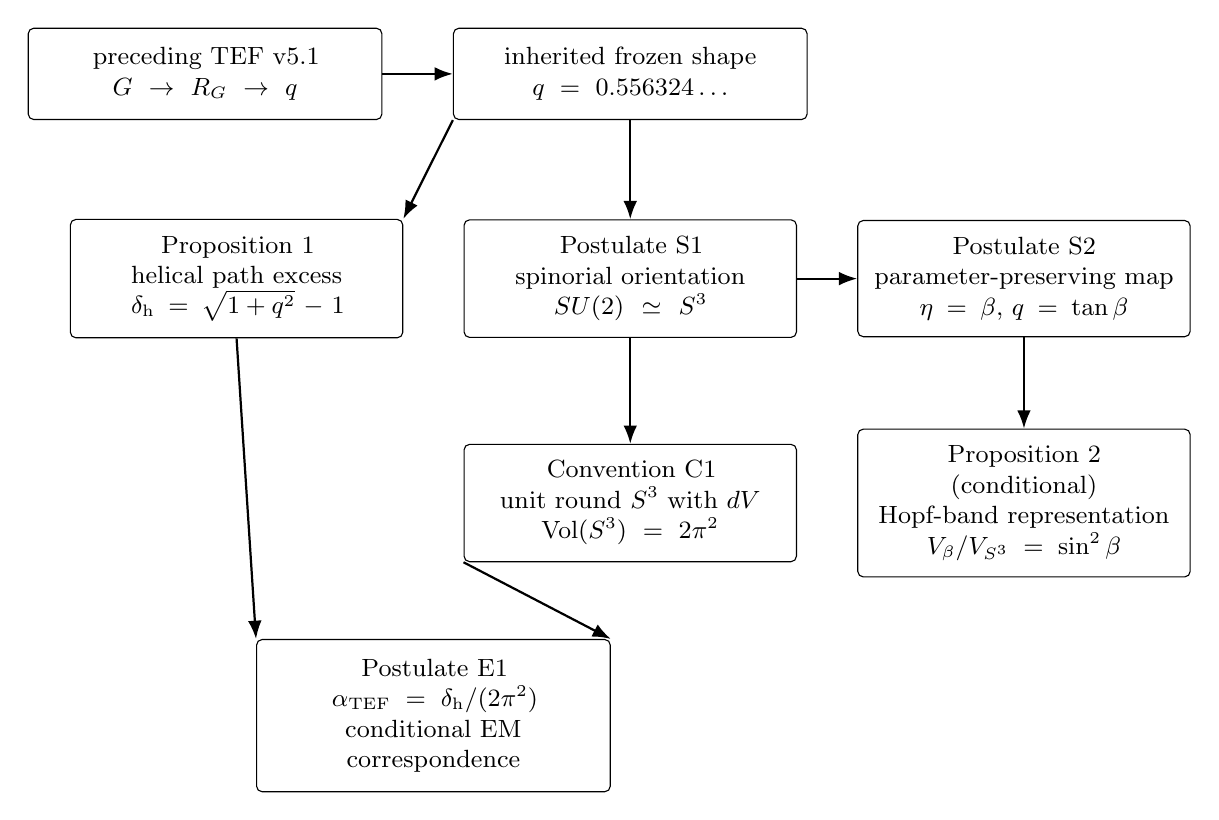
\begin{tikzpicture}[>=Latex,font=\small]
  \tikzset{
    box/.style={draw,rounded corners=2pt,inner sep=7pt,align=center,minimum height=1.02cm,text width=4.0cm},
    sbox/.style={draw,rounded corners=2pt,inner sep=6pt,align=center,minimum height=0.92cm,text width=3.8cm},
    arr/.style={->,thick}
  }

  % Top inheritance chain
  \node[box] (prior) at (-5.4,2.1)
    {preceding TEF v5.1\\$G\to R_G\to q$};
  \node[box] (q) at (0,2.1)
    {inherited frozen shape\\$q=0.556324\ldots$};
  \draw[arr] (prior.east) -- (q.west);

  % First branching level
  \node[sbox] (excess) at (-5.0,-0.5)
    {Proposition 1\\helical path excess\\$\delta_{\rm h}=\sqrt{1+q^2}-1$};
  \node[sbox] (s1) at (0,-0.5)
    {Postulate S1\\spinorial orientation\\$SU(2)\simeq S^3$};
  \node[sbox] (s2) at (5.0,-0.5)
    {Postulate S2\\parameter-preserving map\\$\eta=\beta$, $q=\tan\beta$};

  \draw[arr] (q.south west) -- (excess.north east);
  \draw[arr] (q.south) -- (s1.north);
  \draw[arr] (s1.east) -- (s2.west);

  % Second level: measure convention and conditional weak representation
  \node[sbox] (c1) at (0,-3.35)
    {Convention C1\\unit round $S^3$ with $dV$\\$\Vol(S^3)=2\pi^2$};
  \node[sbox] (weak) at (5.0,-3.35)
    {Proposition 2 (conditional)\\Hopf-band representation\\$V_\beta/V_{S^3}=\sin^2\beta$};

  \draw[arr] (s1.south) -- (c1.north);
  \draw[arr] (s2.south) -- (weak.north);

  % Final electromagnetic postulate: two independent inputs meet without crossings
  \node[box] (e1) at (-2.5,-6.05)
    {Postulate E1\\$\alpha_{\TEF}=\delta_{\rm h}/(2\pi^2)$\\conditional EM correspondence};
  \draw[arr] (excess.south) -- (e1.north west);
  \draw[arr] (c1.south west) -- (e1.north east);
\end{tikzpicture}
\caption{Logical hierarchy of the proposed correspondence.  The upper chain contains only the
previously released TEF input and its inherited helical shape.  The left branch gives the exact
helical path excess.  The central/right branch separates the spinorial completion, the structural
Hopf-coordinate identification, the metric/measure convention, and the conditional weak-angle
representation.  Postulate E1 receives two distinct inputs---the path excess and the chosen
unit-round volume factor---and is therefore displayed separately from Proposition 2.  Straight
arrows denote inheritance, mathematical implication, or an explicitly named modeling choice; they
do not imply that the electromagnetic correspondence has been derived dynamically.}
\label{fig:logic}
\end{figure*}

\section{Discovery-history and mapping-choice burden}

Freezing $q$ before the present calculation removes one important form of fitting, but it does not
remove functional look-elsewhere freedom.  From a single $q$ one can construct many simple
quantities, including $q$, $q^2$, $\sin^2\beta$, $\delta_{\rm h}$, and combinations involving
$\pi$ or group-space measures.  The particular map in Eq.~\eqref{eq:alphacandidate} was recognized
after comparison with the electromagnetic target.  It is therefore not a preregistered or
statistically independent prediction even though $q$ itself was inherited without electromagnetic
reoptimization.

The present paper freezes Eq.~\eqref{eq:alphacandidate} as the object to be tested theoretically.
No multiplicative correction factor is introduced, and no alternative function of $q$ is selected to
remove the residual in Sec.~\ref{sec:comparison}.  The meaningful next question is not whether a
more accurate expression can be guessed, but whether a TEF action can produce this specific map
without post-hoc freedom.

\section{Conditional consequence: a correlated electroweak tuple}
\label{sec:ewseed}

At tree level the electroweak couplings obey
\begin{equation}
e=g\sin\theta_W=g'\cos\theta_W,
\qquad
\tan\theta_W=\frac{g'}{g}.
\label{eq:ewrelations}
\end{equation}
For the following algebraic comparison we use natural units and Heaviside--Lorentz normalization,
$\hbar=c=\varepsilon_0=1$, so $e$ denotes a dimensionless gauge coupling rather than the SI charge
appearing in the opening definition of $\alpha$.

Conditional on both candidate identifications
$\theta_W\rightarrow\beta$ and $\alpha\rightarrow\alpha_{\TEF}$, define
\begin{align}
e_{\geom}&\equiv\sqrt{4\pi\alpha_{\TEF}}
=0.3031251329\ldots,\\
g_{\geom}&\equiv\frac{e_{\geom}}{\sin\beta}
=0.6235139813\ldots,\\
g'_{\geom}&\equiv\frac{e_{\geom}}{\cos\beta}
=0.3468759044\ldots.
\label{eq:geomcouplings}
\end{align}
These are not three additional independent predictions.  They are algebraic descendants of the two
conditional inputs $(\alpha_{\TEF},\beta)$.  Their value is instead one of consistency: any future
TEF matching or running mechanism must transform the correlated set jointly rather than repair the
fine-structure and weak-angle correspondences independently.

For orientation, current precision electroweak analyses quote scheme-dependent quantities near the
$Z$ scale such as \cite{PDG2026}
\begin{equation}
\hat\alpha^{(5)}(M_Z^2)^{-1}\simeq127.93,
\qquad
\sin^2\hat\theta_W(M_Z)\simeq0.23122.
\label{eq:pdgbench}
\end{equation}
These are not direct targets for Eq.~\eqref{eq:alphacandidate}; they illustrate why a genuine
boundary-condition interpretation requires a unique scale, scheme, threshold prescription, and beta
functions.

\begin{table}[t]
\centering
\caption{Quantities generated after the stated conditional identifications.  The last three rows are
algebraically correlated descendants, not independent predictions.}
\label{tab:seed}
\begin{tabular}{@{}ll@{}}
\toprule
Quantity & Geometric value \\
\midrule
$q$ & $0.556324180045$ \\
$\beta$ & $29.0882455^\circ$ \\
$\sin^2\beta$ & $0.2363477652$ \\
$\delta_{\rm h}$ & $0.144332378858$ \\
$\alpha_{\TEF}$ & $0.0073119637319$ \\
$\alpha_{\TEF}^{-1}$ & $136.7621663$ \\
$e_{\geom}$ & $0.3031251329$ \\
$g_{\geom}$ & $0.6235139813$ \\
$g'_{\geom}$ & $0.3468759044$ \\
\bottomrule
\end{tabular}
\end{table}

\section{Empirical comparison}
\label{sec:comparison}

Postulate E1 gives
\begin{align}
\alpha_{\TEF}&=0.007311963731910\ldots,\\
\alpha_{\TEF}^{-1}&=136.76216631599\ldots.
\end{align}
Relative to the 2022 CODATA recommended value in Eq.~\eqref{eq:alpha0},
\begin{equation}
\frac{\alpha_{\TEF}-\alpha(0)}{\alpha(0)}
=2.00225595\times10^{-3},
\label{eq:discrepancy}
\end{equation}
or approximately $0.2002256\%$.  This is vastly larger than the uncertainty in the CODATA
recommended value and the spread relevant to current precision determinations.  Therefore
Eq.~\eqref{eq:alphacandidate} is not a precision prediction of the measured Thomson-limit coupling.

The scale of the discrepancy can also be compared with direct atom-recoil determinations.  Parker
\emph{et al.} obtained $\alpha^{-1}=137.035999046(27)$ from cesium recoil interferometry
\cite{Parker2018}, whereas Morel \emph{et al.} obtained
$\alpha^{-1}=137.035999206(11)$ from rubidium recoil \cite{Morel2020}.  The two determinations
showed a statistically significant tension at their quoted precision, yet their absolute spread is
still negligible compared with the $0.2002\%$ TEF residual.  That metrological tension therefore
cannot be invoked as an explanation of Eq.~\eqref{eq:discrepancy}.

The residual is left unchanged.  We do not introduce an empirical multiplier, alter $q$, change the
$S^3$ radius to force agreement, or choose a running scale after inspection of the data.  Any future
claim that Eq.~\eqref{eq:alphacandidate} is a boundary value rather than a low-energy value must
supply the matching calculation independently.

\section{Relation to current approaches}

The idea that gauge couplings might be calculable from ultraviolet physics is not unique to TEF.
Eichhorn, Held, and Wetterich showed that asymptotically safe quantum-gravity effects can, for
suitable matter content, generate predictive gauge-coupling behavior \cite{EichhornHeldWetterich}.
Giacometti \emph{et al.} have recently revisited gravitational contributions to gauge and Yukawa
beta functions within a proper-time functional flow, explicitly studying gauge-fixing and regulator
dependence \cite{Giacometti2026}.  Recent work has also explored emergent gauge symmetry and
pre-geometric routes to spacetime and gravity \cite{Bass2026,Addazi2024,Addazi2025}.  These
programs differ substantially from TEF in dynamics and mathematical structure; they provide context
for the type of ultraviolet question, not support for the present ansatz.

At the opposite, infrared end of the problem, first-principles lattice-QCD calculations now track the
hadronic running of both the electromagnetic coupling and the weak mixing angle in the same set of
vacuum-polarization observables \cite{Ce2022,Conigli2026}.  This is especially relevant to the
correlated TEF tuple in Sec.~\ref{sec:ewseed}: mainstream precision theory treats the two quantities
as jointly scale-dependent electroweak observables.  A viable TEF boundary-condition interpretation
would therefore need to match and run them together, rather than using separate phenomenological
corrections.

Closer to electroweak numerical structure, Meinert and Hofmann obtain approximate electroweak
parameters from mixed $SU(2)$ Yang--Mills thermodynamics \cite{MeinertHofmann2024}; Monjo has
studied the weak mixing angle within a $U(1,3)$ colored-gravity construction \cite{Monjo2025};
Ciborowski investigates geometric constructibility patterns involving electroweak couplings
\cite{Ciborowski2025}; and Singh places fine-structure and weak-sector normalization in a common
octonionic gauge-coupling ledger \cite{Singh2026}.  Their ontologies and mechanisms are distinct.
The present paper claims only a specific conditional map from one earlier gravity-calibrated helical
shape to an electromagnetic numerical correspondence.

\section{Open dynamical problem and failure conditions}
\label{sec:dynamics}

The correspondence in Eq.~\eqref{eq:alphacandidate} becomes a physical theory only if a future
TEF dynamics removes the conventions and mapping choices exposed above.  A schematic target has
the form
\begin{align}
S_{\TEF}=\int d^4x\,d\mu(U)\Bigl[
&\mathcal L_{\rm frame}(q,U)\notag\\
&-\frac{1}{4g_*^2}\mathcal K_{ab}(q,U)
F^a_{\mu\nu}F^{b\mu\nu}+\cdots\Bigr].
\label{eq:targetaction}
\end{align}
Equation~\eqref{eq:targetaction} is not a proposed completed action; it states what the missing
calculation must eventually accomplish.  In particular, the theory would need to determine:
(i) whether the relevant framed configuration space is indeed $SU(2)$;
(ii) the metric and physical scale on that space;
(iii) the invariant measure and field representations;
(iv) canonical mode normalization;
(v) the coefficient of the four-dimensional gauge kinetic term;
(vi) the relation between the electromagnetic and weak gauge sectors; and
(vii) a common renormalization-group and threshold-matching map.

The present correspondence has explicit theoretical failure conditions.  It fails as an explanation
of $\alpha$ if no consistent TEF action produces Postulate E1, if the physically selected metric or
measure removes the proposed factor, if the $\eta=\beta$ identification cannot be derived from the
framed geometry, or if a unique joint electroweak matching map conflicts with experiment.
Quantitative experimental falsifiability as an electroweak boundary condition requires those missing
scale, scheme, and RG specifications first.

\section{Logical status of the result}

The hierarchy of the present paper is intentionally explicit:
\begin{center}
\small
\begin{tabular}{@{}p{0.30\columnwidth}p{0.62\columnwidth}@{}}
Inherited result & gravity-calibrated $q$ from Ref.~\cite{WuCompanion} \\
Exact geometry & $\delta_{\rm h}=\sqrt{1+q^2}-1$ \\
Postulate S1 & framed $SU(2)\simeq S^3$ completion \\
Postulate S2 & parameter-preserving $\eta=\beta$ map \\
Exact consequence & $V_\beta/V_{S^3}=\sin^2\beta$ \\
Convention C1 & unit round metric, unnormalized $dV$ \\
Postulate E1 & $\alpha_{\TEF}=\delta_{\rm h}/(2\pi^2)$ \\
Conditional consequence & correlated electroweak tuple \\
\end{tabular}
\end{center}
This separation is important methodologically.  The paper does not derive the fine-structure constant.
It identifies a compact numerical correspondence whose upstream geometric parameter is already fixed
by an earlier gravity-calibrated ansatz, and it states precisely which additional assumptions are needed
to turn that correspondence into physics.

\section{Conclusion}

The preceding TEF construction fixes a dimensionless helical shape through the chain
\begin{equation}
G_{\Exp}\to R_G\to q,
\qquad
q\sqrt{1+q^2}=\frac{2}{\pi},
\end{equation}
without electroweak input.  The present paper shows that the same $q$ generates the scale-free
helical path excess
\begin{equation}
\delta_{\rm h}=\sqrt{1+q^2}-1
\end{equation}
and, conditional on a spinorial $SU(2)\simeq S^3$ completion together with the minimal
identification $\eta=\beta$, gives the exact Hopf-band representation
\begin{equation}
\frac{V_\beta}{V_{S^3}}=\sin^2\beta.
\end{equation}

Under the additional and explicitly named electromagnetic Postulate E1,
\begin{equation}
\boxed{
\alpha_{\TEF}=\frac{\sqrt{1+q^2}-1}{2\pi^2},
}
\end{equation}
which yields $\alpha_{\TEF}^{-1}=136.7621663\ldots$.  The result lies about $0.2002\%$ from the
2022 CODATA recommended low-energy value.  No correction is applied.

The main conclusion is therefore not that the fine-structure constant has been derived.  It is that an
earlier, publicly frozen, gravity-calibrated helical parameter admits a particularly compact conditional
map to the electromagnetic numerical regime.  Before the gravity calibration is imposed the map may
be written as $\alpha_{\TEF}(G,h,c;R)$ through Eq.~\eqref{eq:alphaG}; after calibration, the dimensional
constants cancel and the same proposal is most cleanly expressed as $\alpha_{\TEF}=F(q)$.  Whether this
is a physically meaningful bridge from gravity-calibrated microscopic geometry to electroweak coupling,
or only a structured numerical coincidence, is now reduced to a concrete dynamical question: can the
orientation space, metric, measure, gauge kinetic normalization, and joint electroweak matching be
derived from one TEF action?

\section*{Acknowledgments}
The author thanks the broader precision-measurement and theoretical-physics communities whose open
reference data and explicit field-theoretic standards make speculative geometric correspondences
quantitatively testable.

\balance
\begin{thebibliography}{99}

\bibitem{WuCompanion}
X.~Wu,
``A Helical Spacetime Ansatz Linking the Planck Scale and Electroweak Mixing,''
TEF preprint, version 5.1 (2026),
\href{https://doi.org/10.5281/zenodo.22101000}{doi:10.5281/zenodo.22101000}.

\bibitem{Mohr2025}
P.~J. Mohr, D.~B. Newell, B.~N. Taylor, and E.~Tiesinga,
``CODATA recommended values of the fundamental physical constants: 2022,''
\emph{Rev. Mod. Phys.} \textbf{97}, 025002 (2025).
\href{https://doi.org/10.1103/RevModPhys.97.025002}{doi:10.1103/RevModPhys.97.025002}.

\bibitem{NISTalpha}
National Institute of Standards and Technology,
``CODATA Value: inverse fine-structure constant,'' 2022 CODATA recommended value,
\url{https://physics.nist.gov/cgi-bin/cuu/Value?alphinv}.

\bibitem{PDG2026}
J.~de Blas, S.~Dittmaier, and R.~Kogler,
``Electroweak Model and Constraints on New Physics,''
in F.~Takahashi \emph{et al.} (Particle Data Group),
\emph{Review of Particle Physics}, \emph{Int. J. Mod. Phys. A} \textbf{41}, 2630011 (2026),
\url{https://pdg.lbl.gov/2026/reviews/rpp2026-rev-standard-model.pdf}.

\bibitem{Parker2018}
R.~H. Parker, C.~Yu, W.~Zhong, B.~Estey, and H.~M\"uller,
``Measurement of the fine-structure constant as a test of the Standard Model,''
\emph{Science} \textbf{360}, 191--195 (2018).
\href{https://doi.org/10.1126/science.aap7706}{doi:10.1126/science.aap7706}.

\bibitem{Morel2020}
L.~Morel, Z.~Yao, P.~Clad\'e, and S.~Guellati-Kh\'elifa,
``Determination of the fine-structure constant with an accuracy of 81 parts per trillion,''
\emph{Nature} \textbf{588}, 61--65 (2020).
\href{https://doi.org/10.1038/s41586-020-2964-7}{doi:10.1038/s41586-020-2964-7}.

\bibitem{Ce2022}
M.~C\`e, A.~G\'erardin, G.~von Hippel, H.~B. Meyer, K.~Miura, K.~Ottnad,
A.~Risch, T.~San Jos\'e, J.~Wilhelm, and H.~Wittig,
``The hadronic running of the electromagnetic coupling and the electroweak mixing angle from lattice QCD,''
\emph{J. High Energy Phys.} \textbf{08}, 220 (2022), arXiv:2203.08676.
\href{https://doi.org/10.1007/JHEP08(2022)220}{doi:10.1007/JHEP08(2022)220}.

\bibitem{Conigli2026}
A.~Conigli, D.~Djukanovic, G.~von Hippel, S.~Kuberski, H.~B. Meyer, K.~Miura,
K.~Ottnad, A.~Risch, and H.~Wittig,
``The running of the electroweak gauge couplings from first principles,''
arXiv:2607.03370 [hep-lat] (2026).
\href{https://arxiv.org/abs/2607.03370}{arXiv:2607.03370}.

\bibitem{Nakahara2003}
M.~Nakahara,
\emph{Geometry, Topology and Physics}, 2nd ed.
(Institute of Physics Publishing, Bristol, 2003).

\bibitem{EichhornHeldWetterich}
A.~Eichhorn, A.~Held, and C.~Wetterich,
``Quantum-gravity predictions for the fine-structure constant,''
\emph{Phys. Lett. B} \textbf{782}, 198--201 (2018),
arXiv:1711.02949.

\bibitem{Giacometti2026}
G.~Giacometti, K.~Kowalska, D.~Rizzo, E.~M. Sessolo, and D.~Zappal\`a,
``Quantum gravity contributions to the gauge and Yukawa couplings in proper time flow,''
\emph{Phys. Rev. D} \textbf{114}, 016020 (2026), arXiv:2604.03033.
\href{https://doi.org/10.1103/xyg5-lvq4}{doi:10.1103/xyg5-lvq4}.

\bibitem{Bass2026}
S.~D. Bass,
``Emergent Gauge Symmetries in Particle Physics and Cosmology,''
arXiv:2606.19403 (2026).

\bibitem{Addazi2024}
A.~Addazi,
``Gravity from Pre-geometry,''
arXiv:2409.02200 (2024).

\bibitem{Addazi2025}
A.~Addazi,
``Emergent Gravity from a Spontaneously Broken Gauge Symmetry:
a Pre-geometric Prospective,''
arXiv:2512.20681 (2025).

\bibitem{Robertson1971}
B.~Robertson,
``Wyler's Expression for the Fine-Structure Constant,''
\emph{Phys. Rev. Lett.} \textbf{27}, 1545--1547 (1971).
\href{https://doi.org/10.1103/PhysRevLett.27.1545}{doi:10.1103/PhysRevLett.27.1545}.

\bibitem{MeinertHofmann2024}
J.~Meinert and R.~Hofmann,
``Electroweak Parameters from Mixed $SU(2)$ Yang--Mills Thermodynamics,''
\emph{Symmetry} \textbf{16}, 1587 (2024), arXiv:2401.03243.

\bibitem{Monjo2025}
R.~Monjo,
``Weak mixing angle under $U(1,3)$ colored gravity,''
arXiv:2502.11236 (2025).

\bibitem{Ciborowski2025}
J.~Ciborowski,
``Bi-Constructible pattern of weak and flavour mixing: implications for electroweak
coupling constants,''
arXiv:2508.00030 (2025).

\bibitem{Singh2026}
T.~P. Singh,
``Gauge couplings of the Standard Model in the octonionic framework: invariant
normalisations, a conditional weak-sector completion, and a scale-explicit matching
ledger,''
arXiv:2603.28810 (2026).

\end{thebibliography}

\end{document}
